\chapter{関数適用の評価\hspace{-3mm}}

この章では関数型言語で大きな位置を占める関数適用の評価方法を学びます。関数適用とは関数に引数を渡して評価することを言います。前章では組み込み関数である{\tt :+}に2つの引数を与え適用した結果として、それらの和を評価値とする関数適用を見てきました。この章では、自分で作った関数についてその適用を考えてみます。

具体的なターゲットは、次のプログラムです。

\begin{lstlisting}
[[:lambda, [:x, :y], [:+, :x, :y]],
         3, 2]
\end{lstlisting}

これは何でしょうか。次のRubyのプログラムはどうでしょう。
\begin{lstlisting}
def add(x, y)
    x + y
end
add(3, 2)
\end{lstlisting}
いずれも、引数を二つとりその和を値とする関数を用意し、その関数に引数3と2を与えて関数適用しているプログラムです。異なる点は、最初のプログラムの関数は名前を持っていません。言わば、関数の中身そのものです。もう少し詳しく説明すると、{\tt [:lambda, [$<parameters>$], $<body>$]}は仮引数{\tt $<parameters>$}でボディが{\tt $<body>$}の関数です。これを関数として、引数を与えることで、前章で学んだ組み込み関数{\tt :+}と同様に関数適用することができます。

このプログラムを実行するためにはどうすれば良いでしょうか。“引数の3, 2を仮引数の{\tt x}, {\tt y}にそれぞれ代入して、中のプログラムを評価する”と考える人が多いのではないでしょうか。おおよそ正しいのですが、考慮すべきポイントがあります。それを見ていきましょう。


\section{環境}
次のプログラムを考えます。

\begin{lstlisting}
[[:lambda, [:x],
  [:+, 
   [[:lambda, [:x], :x], 2],
   :x]], 
 1]
\end{lstlisting}

この時、上の説明でうまくいくか考えて見ましょう。一番外側の{\tt :lambda}の関数適用から考えていきます。{\tt :x}を1に束縛して、{\tt :+}から始まるカッコの中の式を評価します。最初に関数{\tt :+}を評価して、次に3行目の{\tt :lambda}を評価します。この関数は引数をそのまま返しますので、{\tt :x}を2に束縛して関数適用すると2が返ります。問題は次に評価する4行目の{\tt :x}です。この{\tt :x}は1を返すべきですが、{\tt :x}は先ほど2に束縛しています。その結果、2+2すなわち答えが4となってしまうのです(図 \ref{fig:environment1})。

\begin{figure}[htbp]
\begin{center}
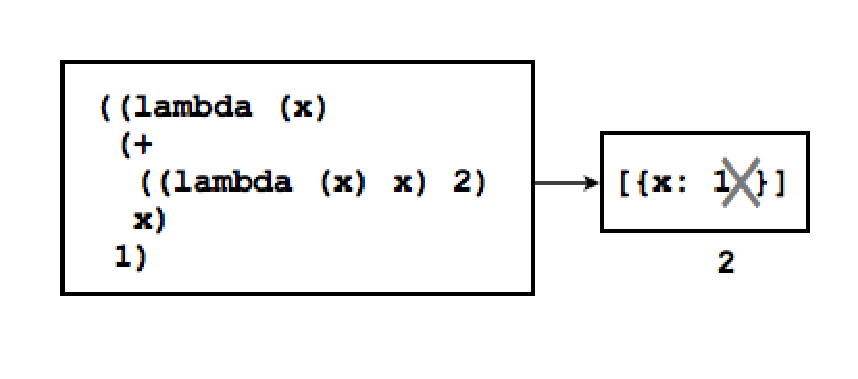
\includegraphics[width=80mm]{images/environment1.eps}
\end{center}
\caption{変数の値を上書きするモデルでの評価のようす。xの値が上書きされるため欲しい値が得られない。}
\label{fig:environment1}
\end{figure}


% \begin{boxnote}
% {\bf コラム: 束縛とは} \\
\begin{breakitembox}[l]{\bf コラム: 束縛とは} 
“{\tt :x}を1に束縛して”という文章が出てきましたが、“束縛”とは何でしょう。変数{\tt :x}と値1とを関連付けるという意味で代入と同じ意味を持ちますが、関数型言語で代入は副作用を引き起こすもの(今は分からないかもしれませんが環境を破壊することとも言います)のことを指すのでそれとは区別して、このように呼びます。また、変数を値に束縛する(bind variable to value)という表現に注意してください。値に対してその名前を一時的につけておいて、後でその名前を通じて値を参照するという使い方をイメージすると良いかもしれません。少し抽象的すぎると思われる人は、Rubyのハッシュを思い出すと良いかもしれません。{\tt h = \{x:1\}}は1という値にxという名前を関連付けておき、後に1を取り出したいときに名前xを使って{\tt h[:x]}という形で取り出すことができます。実際、後に出てくるように$\mu$SchemeRでは変数の束縛をハッシュを用いて実装しています。
% \end{boxnote}
\end{breakitembox}

ところで先ほど、“{\tt :x}は1を返すべき”と言いましたが、なぜでしょう。次のプログラムは上のプログラムの内側のλ式の{\tt :x}を{\tt :y}に変えたものです。

\begin{lstlisting}
[[:lambda, [:x],
  [:+, 
   [[:lambda, [:y], :y], 2],
   :x]], 1]
\end{lstlisting}

このプログラムでは明かに求める答えは3です。プログラミング言語にはスコープという考え方があり変数の有効な範囲が決まっています。多くのプログラミング言語では、今回同様、変数の名前を変えただけでプログラムの結果が変わってほしくないので、{\tt :x}は1を返すような言語仕様になっています。今回作成するプログラミング言語もそのような仕様とします。

話を元に戻しましょう。さて、先ほどの答えが4になってしまう問題を解決する
ためにはどうすれば良いのでしょうか。すでにお気づきかもしれませんが、内
側の{\tt :lambda}の{\tt :x}と外側の{\tt :lambda}の{\tt :x}を区別すれば良いのです。内
側の{\tt :lambda}の関数適用を評価しているときは{\tt :x}を2に束縛し、そ
の外側では{\tt :x}を1に束縛するようにします。具体的には、外側
の{\tt :lambda}の関数適用を評価し始めるときに{\tt :x}を1に束縛します。内側の{\tt
:lambda}の関数適用を評価し始めるときに{\tt :x}を2に束縛する環境を新たに用意してそちらを優先し、
その評価が終わればそれを破棄して元の環境に戻すことで、引き続き{\tt :x}を1に束
縛した環境を使うことが出来ます(図 \ref{fig:environment2}\footnote{あまり本質的なところではありませんが、本書のプログラムでは、配列のコピーが作られるため、\{x:1\}の実体は共通ではありません。})。

\begin{figure}[htbp]
\begin{center}
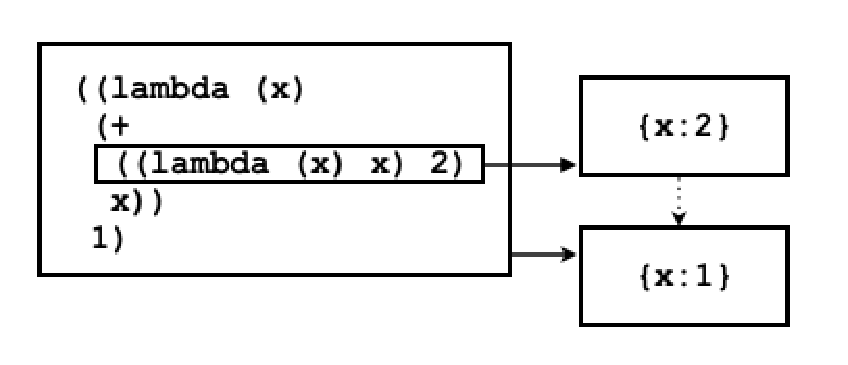
\includegraphics[width=80mm]{images/environment2.eps}
\end{center}
\caption{環境モデル。関数適用時に環境を拡張することで、スコープに応じて、変数が束縛している値を得ることができる。}
\label{fig:environment2}
\end{figure}

ここで新しく環境という言葉を使いました。
環境とは、変数とそれに束縛されている値の組のリストのことです。ここでは、
\{x:1, y:2\}などと表記してxを1にyを2に束縛していることを表し、その組の
リスト[\{x:1, y:2\}, \{x:3\}]で環境を表現することとします。この表現方法
を使えば、最初の{\tt :lambda}を評価しはじめるときは[\{x:1\}]の環境で評価し、
内側の{\tt :lambda}を評価するときは[\{x:2\}, \{x:1\}]という環境で評価します。た
だし同じ変数があった場合、先頭から見ていき最初にマッチした変数に束縛さ
れた値を採用するものとします。内側の{\tt :lambda}を評価した後は[\{x:1\}]
という環境に戻すことで、欲しい値が得られることになります。関数呼び出
し時に仮引数と引数の組を環境のスタックに積み、呼び出し終了時にスタック
から取り出すいうイメージです。

以降、環境に関するRubyプログラムを定義していきます。

{\tt lookup\_var}は与えられた環境の中で、指定した変数が束縛している値を見つける関数です。

\begin{lstlisting}
def lookup_var(var, env)
  alist = env.find{|alist| alist.key?(var)}
  if alist == nil
    raise "couldn't find value to variables:'#{var}'"
  end
  alist[var]
end  
\end{lstlisting}

環境の拡張は、与えられた変数をキーに値を格納したハッシュを作り、それを環境の先頭に追加することで実現します。

\begin{lstlisting}
def extend_env(parameters, args, env)
  alist = parameters.zip(args)
  h = Hash.new
  alist.each { |k, v| h[k] = v }
  [h] + env
end
\end{lstlisting}

\section{let式}

少し遠回りになりますが、ここでプログラムを見やすくするためにlet式というものを導入することにします。

\begin{lstlisting}
[:let, [[:x, 3], [:y, 2]],
 [:+, :x, :y]]
\end{lstlisting}

このプログラムは{\tt :x}を3に束縛し、{\tt :y}を2に束縛した環境で、{\tt [:+, :x, :y]}を評価し、その結果をlet式の評価値とする、と解釈します。λ式とどこが違うんだと思うかもしれませんが、そのとおり同じものです。上のlet式は、下の式と同じ意味です。

\begin{lstlisting}
[[:lambda, [:x, :y], [:+, :x, :y]], 3, 2]
\end{lstlisting}

単にプログラムの見やすさから導入した構文ですので、その評価方法も単純です。
{\tt let}は式から仮引数、引数、評価する式を取り出し、λ式に書き換え、評価した値を返します。

\begin{lstlisting}
def eval_let(exp, env)
  parameters, args, body = let_to_parameters_args_body(exp)
  new_exp = [[:lambda, parameters, body]] + args
  _eval(new_exp, env)
end
\end{lstlisting}

{\tt let}から仮引数、引数ならびに評価する本体の式を抜き出します。

\begin{lstlisting}
def let_to_parameters_args_body(exp)
  [exp[1].map{|e| e[0]}, exp[1].map{|e| e[1]}, exp[2]]
end
\end{lstlisting}

let式かを判定する関数も用意しておきます。

\begin{lstlisting}
def let?(exp)
  exp[0] == :let
end
\end{lstlisting}

\section{クロージャ}

それでは覚えたてのlet式を使って次のプログラムを考えてみます。

\begin{lstlisting}
[:let, [[:x, 2]],
 [:let, [[:fun, [:lambda, [], :x]]],
  [:let, [[:x, 1]],
   [:fun]]]]
\end{lstlisting}

このプログラムの結果、どのような答えが返ってきて欲しいですか。まだ{\tt let}に慣れていない人のために読み方を補足すると、{\tt :x}を2に束縛した環境で、{\tt :fun}を{\tt :x}を返す関数に束縛した環境で、{\tt :x}を1に束縛した環境で、{\tt :fun}関数を適用した値を求める、というプログラムです。要は{\tt :x}が{\tt fun:}の呼び出し時の値をとるのか(この場合{\tt :x}は1です)、評価されたときの値をとるのか(この場合{\tt :x}は2です)です。正解は、“プログラミング言語を作る人(すなわち、著者!)が決める"です。そして、その答えは、2です\footnote{このようにプログラムの文脈だけで値を決められるスコープをレキシカルスコープと言い、一方で1が返るようなプログラム実行時の環境を利用する方法をダイナミックスコープと言います。}。

では2を得るためには、どう実現すれば良いでしょう。

λ式を評価するときに、評価時の環境も合わせて持っておくことで、これを実現出来ます。
λ式を評価した時にその結果として、λ式とその時の環境をペア([$lambda () x$, [\{x:2\}]])で持ち、{\tt fun}はこれを値として束縛します。その後{\tt :x}が1を束縛すると、環境は[\{x:1\}, \{x:2\}]となります。ただし、{\tt fun}を関数適用する際には、先ほどのペアで作成した環境[\{x:2\}]を利用してλ式を評価することで{\tt x}の値は2となります。

まとめると、λ式の評価値はλ式とその評価時の環境のペアです。そのλ式を
関数適用する際には、もう一方のペアである環境で(引数を仮引数に束縛して拡
張して)評価します。このλ式と環境のペアのことをクロージャと呼びます。

実際のRubyのプログラムで実現していきます。

λ式は、λ式と環境でクロージャを作りその評価値とします。

\begin{lstlisting}
def eval_lambda(exp, env)
  make_closure(exp, env)
end

def make_closure(exp, env)
  parameters, body = exp[1], exp[2]
  [:closure, parameters, body, env]
end
\end{lstlisting}

λ式の関数適用は、クロージャからλ式と仮引数および環境を取り出し、取り出した環境を引数と仮引数で拡張して、λ式を評価します。

\begin{lstlisting}
def lambda_apply(closure, args)
  parameters, body, env = closure_to_parameters_body_env(closure)
  new_env = extend_env(parameters, args, env)
  _eval(body, new_env)
end

def closure_to_parameters_body_env(closure)
  [closure[1], closure[2], closure[3]]
end
\end{lstlisting}

最後に、{\tt \_eval}を変更します。式に加えて環境も引数とします。その他、導入したλ式やlet式を扱えるよう変更します。{\tt apply}もλ式の関数適用を扱えるように変更します。

\begin{lstlisting}
def _eval(exp, env)
  if not list?(exp)
    if immediate_val?(exp)
      exp
    else 
      lookup_var(exp, env)
    end
  else
    if special_form?(exp)
      eval_special_form(exp, env)
    else
      fun = _eval(car(exp), env)
      args = eval_list(cdr(exp), env)
      apply(fun, args)
    end
  end
end

def special_form?(exp)
  lambda?(exp) or 
    let?(exp)
end

def lambda?(exp)
  exp[0] == :lambda
end

def eval_special_form(exp, env)
  if lambda?(exp)
    eval_lambda(exp, env)
  elsif let?(exp)
    eval_let(exp, env)
  end
end

def eval_list(exp, env)
  exp.map{|e| _eval(e, env)}
end    

def apply(fun, args)
  if primitive_fun?(fun)
    apply_primitive_fun(fun, args)
  else
    lambda_apply(fun, args)
  end
end

def primitive_fun?(exp)
  exp[0] == :prim
end
\end{lstlisting}

ユーザプログラムの評価に使う大域環境を用意します。大域環境には組み込み関数を設定します。これにより、組み込み関数を変数と同じように{\tt lookup\_var}で扱うことが出来ます。

\begin{lstlisting}
$global_env = [$primitive_fun_env]
\end{lstlisting}

以降、プログラムを評価して下さいと言われた時は、次のようにプログラムと、
この環境を引数として評価して下さい。

\begin{lstlisting}
exp = [[:lambda, [:x, :y], [:+, :x, :y]], 3, 2]
puts _eval(exp, $global_env)
\end{lstlisting}

クロージャは強力です。次のプログラムを見てください。

\begin{lstlisting}
[:let, [[:x, 3]],
 [:let, [[:fun, [:lambda, [:y], [:+, :x, :y]]]],
   [:+, [:fun, 1], [:fun, 2]]]]
\end{lstlisting}

{\tt :fun}を束縛したλ式中の{\tt :x}はその中で値を束縛していないにも関わらず利用できる点に注意して下さい\footnote{p. \pageref{column:closure}でもう少し強力な例を示します。}。これはクロージャが環境を持っているからです。

\section{評価(eval)と関数適用(apply)}

プログラムの評価方法はこれでほぼ全て学びました。流れをおさらいしてみましょう。プログラムが与えられると、関数ならびに引数の部分に分けられそれぞれを評価します。その後、引数をその関数に適用します。すなわち、仮引数を引数に束縛して、関数のボディを評価します。次は、このボディの中に含まれるプログラムについて、これら一連の処理を繰り返すことになります。このように評価(eval)と関数適用(apply)を再帰的に繰り返しながらプログラムは実行されていくのです。


\section{λ式とクロージャの違い}

ここまで読んできた皆さんなら、λ式とクロージャの違いをよく理解しているでしょう。λ式は単なるプログラムのコードであり、クロージャはλ式とそれを評価した時の環境のペアです。λ式を評価するとクロージャがその評価値となります。このクロージャを関数適用するときは、クロージャ中の環境(仮引数を引数に束縛し拡張した環境)でλ式を評価します。

λ式扱うことができるプログラミング言語は、関数を値として扱う関数、すな
わち高階関数としてFORTRANなど古くから存在してきました。値として扱うとは、
引数や返り値などで使うことが出来ることを言います\footnote{専門用語では、
関数がファーストクラスのオブジェクトであるとも言います。}。高階関数は処理を抽
象化できるため強力な機能となります。例えば、関数の積分値を数値計算で求め
たいとき、求める関数を引数とすることで、各関数毎に同じ処理を書かずにす
みますし、記載した処理がわかりやすくなります。

クロージャは高階関数よりもさらに強力です。ソースコードと環境のペアを値として扱うことで、内部状態を隠蔽することが可能です。最近のプログラミング言語ではクロージャを扱えるものが増えています。ぜひ、その可能性を最大限に利用してプログラミングをより楽しんでください。

\section{まとめ}

この章では次のことを学びました。

\begin{itemize}
\item 関数適用の評価方法
\item クロージャの関数適用は、クロージャ中の環境を仮引数を引数に束縛して拡張した上で、λ式を評価する
\item 環境とは、変数とそれに束縛された値の組のリスト
\item クロージャはλ式と評価時の環境のペア
\item プログラムは評価と関数適用が再帰的に呼ばれながら実行される
\end{itemize}


